% =====================================================================
%  第 6 章 形变量子化 —— ch06b（§6.2 末、§6.3、§6.4）
%  页段：PDF 314–334（原书 p.313–333）
%  第 6 章（全书正文）在本块结束
% =====================================================================

% [原文 p.313]
\begin{theorem}{6.2.10（费多谢夫）}
  $(C^\infty(M)[[\lambda]],\ast_D)$ 定义了辛流形 $(M,\omega)$ 上的形变量子化。
\end{theorem}

\begin{proof}
诱导出的乘积 $\ast_D$ 显然是 $\lambda$-线性的，且结合。取 $f,g\in C^\infty(M)$。由逐纤维的 Moyal 乘积，
\[
f\ast_D g=\sigma\bigl(\sigma^{-1}(f)\ast\sigma^{-1}(g)\bigr)=fg+O(\lambda),
\]
故 $\ast_D$ 在 $\lambda\to0$ 时的极限给出经典乘积。

剩下要检验一阶非交换性。令
\[
\sigma^{-1}(f(\mathbf x))=f(\mathbf x)-\sum_i f_i(\mathbf x)y^i
\quad\text{模}\ \mathcal W_2.
\]
平坦性条件 $D(\sigma^{-1}(f))=0$ 蕴含
\[
df(\mathbf x)-\delta\Bigl(\sum_i f_i(\mathbf x)y^i\Bigr)=0
\quad\Longrightarrow\quad
f_i(\mathbf x)=\frac{\partial f}{\partial x^i}.
\]
因此
\begin{align*}
\frac1\lambda[f,g]_{\ast_D}
&=\frac1\lambda\sigma\bigl([\sigma^{-1}(f),\sigma^{-1}(g)]_\ast\bigr)\\
&=\sigma\Bigl(\sum_{i,j}\omega^{ij}(\mathbf x)
\frac{\partial\sigma^{-1}(f)}{\partial y^i}
\frac{\partial\sigma^{-1}(g)}{\partial y^j}+O(\lambda)\Bigr)\\
&=\sum_{i,j}\omega^{ij}(\mathbf x)f_i(\mathbf x)f_j(\mathbf x)+O(\lambda)\\
&=\{f,g\}+O(\lambda),
\end{align*}
这正是所需。
\end{proof}

% [§6.2 的本节重点：本节跨 ch06a/ch06b 两块，takeaway 放在本节真正结束处]
\takeaway{本节用费多谢夫的几何方法构造辛流形上的形变量子化：外尔丛承载逐纤维 Moyal 乘积，辛联络的曲率由阿贝尔联络消去；阿贝尔联络的平坦截面经象征映射等同于形式幂级数，从而给出整体化的星乘积，定理 6.2.10 说明它确实是形变量子化。}

\section{泊松流形}

辛流形上的函数定义了泊松代数。不过，泊松代数可以在更一般的框架中出现，即所谓的泊松流形。这类流形包含一大类重要的例子，例如李代数 $\mathfrak g$ 的对偶 $\mathfrak g^*$，其形变量子化给出泛包络代数 $U(\mathfrak g)$。

\subsection{多向量场}

\begin{definition}{6.3.1}
  设 $M$ 是光滑流形。记
  \[
  \operatorname{PV}^\bullet(M)=\bigoplus_k\operatorname{PV}^k(M),
  \qquad
  \operatorname{PV}^k(M):=\Gamma(M,\wedge^kTM).
  \]
\end{definition}

$\operatorname{PV}^k(M)$ 中的元素称为 $k$-多向量场。对 $\mu\in\operatorname{PV}^k(M)$，记 $|\mu|=k$。$\operatorname{PV}^\bullet(M)$ 在楔积下是分次交换代数：
\[
\alpha\wedge\beta=(-1)^{|\alpha||\beta|}\beta\wedge\alpha.
\]

% [原文 p.314]
对 $k=1$，$\operatorname{PV}^1(M)=\operatorname{Vect}(M)$ 是 $M$ 上的向量场。$\operatorname{Vect}(M)$ 上有一个李括号
\[
[-,-]:\operatorname{Vect}(M)\times\operatorname{Vect}(M)
\longrightarrow\operatorname{Vect}(M).
\]
这个李括号通过下式延拓到多向量场：
\begin{align*}
&[X_1\wedge\cdots\wedge X_m,Y_1\wedge\cdots\wedge Y_n]_{\mathrm{SN}}\\
&\quad:=\sum_{i,j}(-1)^{i+j}[X_i,Y_j]\wedge
X_1\wedge\cdots\wedge\widehat X_i\wedge\cdots\wedge X_m
\wedge Y_1\wedge\cdots\wedge\widehat Y_j\wedge\cdots\wedge Y_n
\end{align*}
以及
\[
[f,X_1\wedge\cdots\wedge X_m]_{\mathrm{SN}}
:=\sum_i(-1)^iX_i(f)X_1\wedge\cdots\wedge\widehat X_i
\wedge\cdots\wedge X_m,
\]
其中 $X_i,Y_j$ 是向量场，$f$ 是函数。这个括号
\[
[-,-]_{\mathrm{SN}}:\operatorname{PV}^k(M)\times\operatorname{PV}^l(M)
\longrightarrow\operatorname{PV}^{k+l-1}(M)
\]
称为斯豪滕–奈恩黑斯括号，也叫斯豪滕括号。

\begin{proposition}{6.3.2}
  斯豪滕–奈恩黑斯括号满足以下性质：
  \begin{itemize}
    \item \emph{斜对称性}
    \[
    [\alpha,\beta]_{\mathrm{SN}}
    =-(-1)^{(|\alpha|-1)(|\beta|-1)}[\beta,\alpha]_{\mathrm{SN}}.
    \]
    \item \emph{莱布尼茨律}
    \[
    [\alpha,\beta\wedge\gamma]_{\mathrm{SN}}
    =[\alpha,\beta]_{\mathrm{SN}}\wedge\gamma
    +(-1)^{(|\alpha|-1)|\beta|}\beta\wedge[\alpha,\gamma]_{\mathrm{SN}}.
    \]
    \item \emph{雅可比恒等式}
    \[
    [[\alpha,\beta]_{\mathrm{SN}},\gamma]_{\mathrm{SN}}
    =[\alpha,[\beta,\gamma]_{\mathrm{SN}}]_{\mathrm{SN}}
    -(-1)^{(|\alpha|-1)(|\beta|-1)}
    [\beta,[\alpha,\gamma]_{\mathrm{SN}}]_{\mathrm{SN}}.
    \]
  \end{itemize}
\end{proposition}

\begin{proof}
  直接计算。
\end{proof}

雅可比恒等式也可写成对称形式
\begin{align*}
&(-1)^{(|\alpha|-1)(|\gamma|-1)}[\alpha,[\beta,\gamma]_{\mathrm{SN}}]_{\mathrm{SN}}
+(-1)^{(|\beta|-1)(|\alpha|-1)}[\beta,[\gamma,\alpha]_{\mathrm{SN}}]_{\mathrm{SN}}\\
&\quad
+(-1)^{(|\gamma|-1)(|\beta|-1)}[\gamma,[\alpha,\beta]_{\mathrm{SN}}]_{\mathrm{SN}}=0.
\end{align*}

\subsection{泊松流形与泊松上同调}

\paragraph{泊松流形}\par

\begin{definition}{6.3.3}
  $M$ 上的泊松双向量是满足
  \[
  [P,P]_{\mathrm{SN}}=0
  \]
  的 $2$-多向量场 $P\in\operatorname{PV}^2(M)$。
\end{definition}

若 $P$ 是泊松双向量，则称对 $(M,P)$ 为泊松流形。

% [原文 p.315]
设 $(M,P)$ 是泊松流形。可以在 $C^\infty(M)$ 上定义泊松括号
\[
\{-,-\}_P:C^\infty(M)\times C^\infty(M)\longrightarrow C^\infty(M)
\]
如下：
\[
\{f,g\}_P:=P(df\otimes dg).
\]
在 $M$ 的局部坐标 $\{x^i\}$ 下，令
\[
P=\frac12\sum_{i,j}P^{ij}(\mathbf x)\partial_{x^i}\wedge\partial_{x^j}.
\]
则
\[
\{f,g\}_P=\sum_{i,j}P^{ij}(\mathbf x)\partial_{x^i}f\partial_{x^j}g.
\]

\begin{proposition}{6.3.4}
  $(C^\infty(M),\{-,-\}_P)$ 定义了泊松代数。$\{-,-\}_P$ 的雅可比恒等式等价于 $[P,P]_{\mathrm{SN}}=0$。
\end{proposition}

\begin{proof}
  我们来检验 $\{-,-\}_P$ 的雅可比恒等式。
  \begin{align*}
  &\{\{f,g\}_P,h\}_P+\text{循环置换}\\
  &\quad=\sum P^{ij}\partial_i\bigl(P^{kl}\partial_kf\partial_lg\bigr)\partial_jh
  +\text{循环置换}\\
  &\quad=\sum P^{ij}\partial_iP^{kl}\partial_kf\partial_lg\partial_jh
  +\text{循环置换}\\
  &\quad=\Bigl(\frac12\sum_{i,j}P^{ij}\partial_iP^{kl}
  \partial_k\wedge\partial_l\wedge\partial_j\Bigr)(df\otimes dg\otimes dh)\\
  &\quad=([P,P]_{\mathrm{SN}})(df\otimes dg\otimes dh).
  \end{align*}
\end{proof}

\begin{example}{6.3.5}
  设 $(M,\omega)$ 是辛流形。在局部坐标下
  \[
  \omega=\frac12\omega_{ij}dx^i\wedge dx^j.
  \]
  设 $\omega^{ij}$ 是 $\omega_{ij}$ 的逆。则
  \[
  \omega^{-1}:=\frac12\sum_{i,j}\omega^{ij}\partial_{x^i}\wedge\partial_{x^j}
  \]
  定义了泊松双向量。泊松括号 $\{-,-\}_{\omega^{-1}}$ 正是辛相空间上的泊松括号。此时
  \[
  d\omega=0\quad\Longleftrightarrow\quad[\omega^{-1},\omega^{-1}]_{\mathrm{SN}}=0.
  \]
\end{example}

\begin{example}{6.3.6（常值泊松结构）}
  设 $M=\R^n$，且
  \[
  P=\frac12\sum_{i,j}P^{ij}\partial_{x^i}\wedge\partial_{x^j},
  \qquad P^{ij}\in\R.
  \]
  由于 $P^{ij}$ 是常数，$[P,P]_{\mathrm{SN}}=0$ 成立。这样的 $P$ 称为常值泊松结构。
\end{example}

% [原文 p.316]
\begin{example}{6.3.7（线性泊松结构）}
  设 $M=\R^n$，且
  \[
  P=\frac12\sum_{i,j}P^{ij}(\mathbf x)\partial_{x^i}\wedge\partial_{x^j},
  \qquad P^{ij}(\mathbf x)=\sum_k c_k^{ij}x^k.
  \]
  这里 $c_k^{ij}\in\R$ 是常数，故 $P^{ij}(\mathbf x)$ 关于 $\mathbf x$ 是线性的。泊松括号为
  \[
  \{x^i,x^j\}_P=\sum_k c_k^{ij}x^k.
  \]
  从这个表达式可以清楚看出，雅可比恒等式等价于 $c_k^{ij}$ 给出某个李代数的结构常数这一条件。

  从内蕴的角度，可以把 $M=\mathfrak g^*$ 等同于李代数 $\mathfrak g$ 的线性对偶。线性坐标 $\{x^i\}$ 可以看作 $\mathfrak g$ 的一组基，李括号在其上通过结构常数 $c_k^{ij}$ 表达。线性泊松结构也称为李–泊松结构。
\end{example}

\paragraph{泊松上同调}\par

设 $(M,P)$ 是泊松流形。定义
\begin{align*}
d_P&:\operatorname{PV}^\bullet(M)\longrightarrow\operatorname{PV}^{\bullet+1}(M),\\
\alpha&\longmapsto[P,\alpha]_{\mathrm{SN}}.
\end{align*}
利用雅可比恒等式
\[
[[P,P]_{\mathrm{SN}},-]_{\mathrm{SN}}=2[P,[P,-]_{\mathrm{SN}}]_{\mathrm{SN}}
\]
以及泊松条件 $[P,P]_{\mathrm{SN}}=0$，可得
\[
d_P^2=0.
\]
于是 $(\operatorname{PV}^\bullet(M),d_P)$ 给出复形
\[
0\longrightarrow\operatorname{PV}^0(M)\xrightarrow{d_P}\operatorname{PV}^1(M)
\xrightarrow{d_P}\cdots\xrightarrow{d_P}\operatorname{PV}^n(M)\longrightarrow0,
\qquad n=\dim M,
\]
它称为利赫内罗维奇复形。

\begin{definition}{6.3.8}
  利赫内罗维奇复形的上同调称为泊松上同调，记作
  \[
  H_P^k(M):=H^k(\operatorname{PV}^\bullet(M),d_P).
  \]
\end{definition}

\begin{example}{6.3.9}
  考虑泊松结构的无穷小形变
  \[
  P\longrightarrow P+\varepsilon Q,\qquad Q\in\operatorname{PV}^2(M),
  \]
  其中 $\varepsilon$ 是无穷小参数。泊松条件在首阶给出
  \[
  [P+\varepsilon Q,P+\varepsilon Q]_{\mathrm{SN}}=2\varepsilon[P,Q]_{\mathrm{SN}}=0,
  \]
  也就是说 $Q$ 是 $d_P$-闭的。设 $X$ 是向量场。它在 $M$ 上生成流，把 $P$ 变为
  \[
  P\longrightarrow P+d_PX.
  \]

% [原文 p.317]
  因此，$d_P$-恰当的 $Q$ 对应由微分同胚诱导的平凡形变。于是
  \[
  H_P^2(M)=\frac{\{\text{$P$ 的一阶形变}\}}{\{\text{平凡形变}\}}.
  \]
\end{example}

\begin{example}{6.3.10}
  设 $(M,\omega)$ 是辛流形，$P$ 是泊松双向量 $P=\omega^{-1}$。$\omega$ 的非退化性诱导出丛同构
  \begin{align*}
  \varphi&:TM\longrightarrow T^*M,\\
  X&\longmapsto-\iota_X\omega.
  \end{align*}
  在局部坐标 $\omega=\frac12\omega_{ij}dx^i\wedge dx^j$ 下，
  \[
  \varphi(\partial_{x^i})=-\sum_j\omega_{ij}dx^j.
  \]
  延拓到外张量，$\varphi$ 诱导出 $k$-多向量场与微分 $k$-形式之间的同构
  \[
  \varphi:\operatorname{PV}^k(M)\longrightarrow\Omega^k(M).
  \]
  注意到
  \begin{itemize}
    \item 对任意函数 $f$，
    \[
    \varphi(d_Pf)=\varphi\Bigl(\sum_{i,j}\omega^{ij}\partial_{x^j}f\partial_{x^i}\Bigr)=df;
    \]
    \item 对向量场 $\partial_{x^k}$，
    \begin{align*}
    \varphi(d_P(\partial_{x^k}))
    &=\varphi\Bigl(-\frac12\sum_{i,j}\partial_k\omega^{ij}
    \partial_{x^i}\wedge\partial_{x^j}\Bigr)\\
    &=-\frac12\sum_{i,j,m,l}\partial_k\omega^{ij}\omega_{im}\omega_{jl}
    dx^m\wedge dx^l\\
    &=\frac12\sum_{i,j,m,l}\partial_k\omega_{im}\omega^{ij}\omega_{jl}
    dx^m\wedge dx^l\\
    &=\frac12\sum_{i,m}\partial_k\omega_{im}dx^m\wedge dx^i\\
    &\overset{\text{用 }d\omega=0}{=}
    -\frac12\sum_{i,m}\bigl(\partial_i\omega_{mk}+\partial_m\omega_{ki}\bigr)
    dx^m\wedge dx^i\\
    &=-d\Bigl(\sum_i\omega_{ki}dx^i\Bigr)\\
    &=d\varphi(\partial_{x^k}).
    \end{align*}
  \end{itemize}

  % [原文 p.318]
  利用莱布尼茨律，可知 $\varphi$ 给出两个复形之间的等同
  \[
  (\operatorname{PV}^\bullet(M),d_P)\xrightarrow{\ \varphi\ }
  (\Omega^\bullet(M),d).
  \]
  特别地，有
  \[
  H_{\omega^{-1}}^2(M)\cong H^2(M).
  \]
  这说明 $\omega^{-1}$ 的泊松形变由 $H^2(M)$ 参数化，也就是由辛形式 $\omega$ 在 $H^2(M)$ 中的形变诱导而来。
\end{example}

\subsection{孔采维奇的星乘积}

\paragraph{星乘积}\par

\begin{definition}{6.3.11}
  设 $(M,P)$ 是泊松流形。$(M,P)$ 上的星乘积（或形变量子化）是 $C^\infty(M)$ 的形式形变 $(C^\infty(M)[[\lambda]],\ast)$
  \[
  f\ast g=f\cdot g+\sum_{k=1}^\infty\lambda^k\mu_k(f,g),
  \]
  使得
  \begin{itemize}
    \item $\displaystyle\lim_{\lambda\to0}\frac1\lambda(f\ast g-g\ast f)=\{f,g\}_P$；
    \item 每个 $\mu_k$ 都是双微分算子。
  \end{itemize}
\end{definition}

换言之，$(M,P)$ 上的星乘积是泊松代数 $(C^\infty(M),\{-,-\}_P)$ 的形变量子化，并且要求所有 $\mu_k$ 都是「局部的」。在具体问题中，$C^\infty(M)$ 也可以换成其他合适的函数（例如多项式、形式幂级数等）。

\begin{example}{6.3.12}
  设 $(M,\omega)$ 是辛流形，$P=\omega^{-1}$。则费多谢夫的阿贝尔联络 $D$ 在 $(M,\omega^{-1})$ 上给出星乘积 $\ast_D$。见 §6.2.5。
\end{example}

\begin{example}{6.3.13}
  设 $M=\R^n$，且
  \[
  P=\frac12\sum_{i,j}P^{ij}\partial_{x^i}\wedge\partial_{x^j},
  \qquad P^{ij}\in\R
  \]
  是常值泊松结构。当 $\det(P^{ij})=0$ 时，$P$ 并不来自辛结构。尽管如此，同样的 Moyal 乘积公式
  \[
  f\ast g:=f\,\ee^{\frac{\lambda}{2}\sum_{i,j}P^{ij}
  \frac{\overleftarrow{\partial}}{\partial x^i}
  \frac{\overleftarrow{\partial}}{\partial x^j}}g
  \]
  在 $(\R^n,P)$ 上定义了星乘积。
\end{example}

\begin{example}{6.3.14}
  设 $\mathfrak g$ 是李代数，$M=\mathfrak g^*$ 带有李–泊松结构 $P_{\mathfrak g}$。令
  \[
  \mathcal U^\lambda(\mathfrak g):=T(\mathfrak g)[\lambda]/\sim,
  \]
  其中 $T(\mathfrak g)=\bigoplus_{m\ge0}\mathfrak g^{\otimes m}$ 是 $\mathfrak g$ 的张量代数，商关系 $\sim$ 为
  \[
  x\otimes y-y\otimes x\sim\lambda[x,y].
  \]
  若取 $\lambda=1$，则 $\mathcal U^{\lambda=1}(\mathfrak g)$ 是 $\mathfrak g$ 的泛包络代数。令
  \[
  \operatorname{Sym}(\mathfrak g):=\bigoplus_{m\ge0}\operatorname{Sym}^m(\mathfrak g)
  =\lim_{\lambda\to0}\mathcal U^\lambda(\mathfrak g)
  \]
  表示 $\mathfrak g^*$ 上的多项式函数环。

% [原文 p.319]
  可以通过对称化映射把 $\operatorname{Sym}(\mathfrak g)$ 嵌入 $\mathcal U^\lambda(\mathfrak g)$：
  \begin{align*}
  \varphi&:\operatorname{Sym}(\mathfrak g)[\lambda]
  \longrightarrow\mathcal U^\lambda(\mathfrak g),\\
  x_1x_2\cdots x_m\lambda^l&\longmapsto
  \frac{\lambda^l}{m!}\sum_{\sigma\in S_m}
  x_{\sigma(1)}\otimes\cdots\otimes x_{\sigma(m)},
  \end{align*}
  由庞加莱–伯克霍夫–维特定理（Poincaré–Birkhoff–Witt 定理），这是向量空间同构。

  $\mathcal U^\lambda(\mathfrak g)$ 以 $\otimes$ 为乘积，是结合代数。这使我们可以在 $\operatorname{Sym}(\mathfrak g)[\lambda]$ 上定义一个典范星乘积 $\ast_{\mathfrak g}$：
  \[
  (f_1\ast_{\mathfrak g}f_2):=\varphi^{-1}\bigl(\varphi(f_1)\otimes\varphi(f_2)\bigr).
  \]
  例如，若 $X,Y\in\mathfrak g$ 是一次元素，则
  \begin{align*}
  X\ast_{\mathfrak g}Y
  &=\varphi^{-1}(X\otimes Y)
  =\varphi^{-1}\Bigl(\frac12(X\otimes Y+Y\otimes X)
  +\frac12(X\otimes Y-Y\otimes X)\Bigr)\\
  &=XY+\frac\lambda2[X,Y],\\[2pt]
  X^2\ast_{\mathfrak g}Y
  &=\varphi^{-1}(X\otimes X\otimes Y)\\
  &=\varphi^{-1}\Bigl(\frac13(X\otimes X\otimes Y+X\otimes Y\otimes X
  +Y\otimes X\otimes X)\\
  &\qquad+\frac23X\otimes(X\otimes Y-Y\otimes X)
  +\frac13\bigl((X\otimes Y-Y\otimes X)\otimes X\bigr)\Bigr)\\
  &=X^2Y+\lambda X[X,Y]+\frac{\lambda^2}{6}[X,[X,Y]].
  \end{align*}

  值得指出，Moyal 乘积公式在这种线性泊松情形下并不适用。上例中的项 $\frac{\lambda^2}{6}[X,[X,Y]]$ 给出了进一步的修正。一般地，Moyal 乘积公式
  \[
  \ee^{\frac{\lambda}{2}\sum_{i,j}
  \frac{\overleftarrow{\partial}}{\partial x^i}P^{ij}(\mathbf x)
  \frac{\overrightarrow{\partial}}{\partial x^j}}
  \]
  在 $P^{ij}(\mathbf x)$ 不是常数时不再结合。这给泊松流形上星乘积的构造带来了重大困难。
\end{example}

\begin{example}{6.3.15}
  设 $M=\R^2$，$P=xy\partial_x\wedge\partial_y$。记
  \[
  \partial_{\log x}:=x\partial_x,\qquad \partial_{\log y}:=y\partial_y.
  \]
  于是可以把 $P$ 写成
  \[
  P=\partial_{\log x}\wedge\partial_{\log y}.
  \]
  由此可知
  \[
  f\ast g:=f\,\ee^{\frac{\lambda}{2}\bigl(
  \overleftarrow{\partial_{\log x}}\overrightarrow{\partial_{\log y}}
  -\overleftarrow{\partial_{\log y}}\overrightarrow{\partial_{\log x}}\bigr)}g
  \]
  在 $(\R^2,P)$ 上定义了星乘积。在这个星乘积下
  \begin{align*}
  x\ast y&=\ee^{\frac\lambda2}xy,\\
  y\ast x&=\ee^{-\frac\lambda2}xy.
  \end{align*}
  特别地，得到
  \[
  x\ast y=\ee^\lambda y\ast x.
  \]
\end{example}

\paragraph{孔采维奇的星乘积}\par

在 [37] 中，孔采维奇利用二维泊松 $\sigma$-模型的量子场论，给出了一个把 Moyal 乘积公式修正为结合乘法的显著显式方法（后来由 Cattaneo–Felder [8] 解释）。

% [原文 p.320]
\begin{theorem}{6.3.16（孔采维奇）}
  任何泊松流形上都存在形变量子化。
\end{theorem}

我们简述孔采维奇构造的基本想法。考虑泊松流形
\[
\Bigl(\R^n,\;P=\frac12\sum_{i,j}P^{ij}(\mathbf x)
\partial_{x^i}\wedge\partial_{x^j}\Bigr).
\]
设 $\Gamma_r$ 是画在上半平面内、有 $r+2$ 个顶点和 $2r$ 条（有向）边的图，其中两个顶点放在实轴上且只有入边，其余 $r$ 个顶点放在内部且每个都有两条出边。

\begin{center}
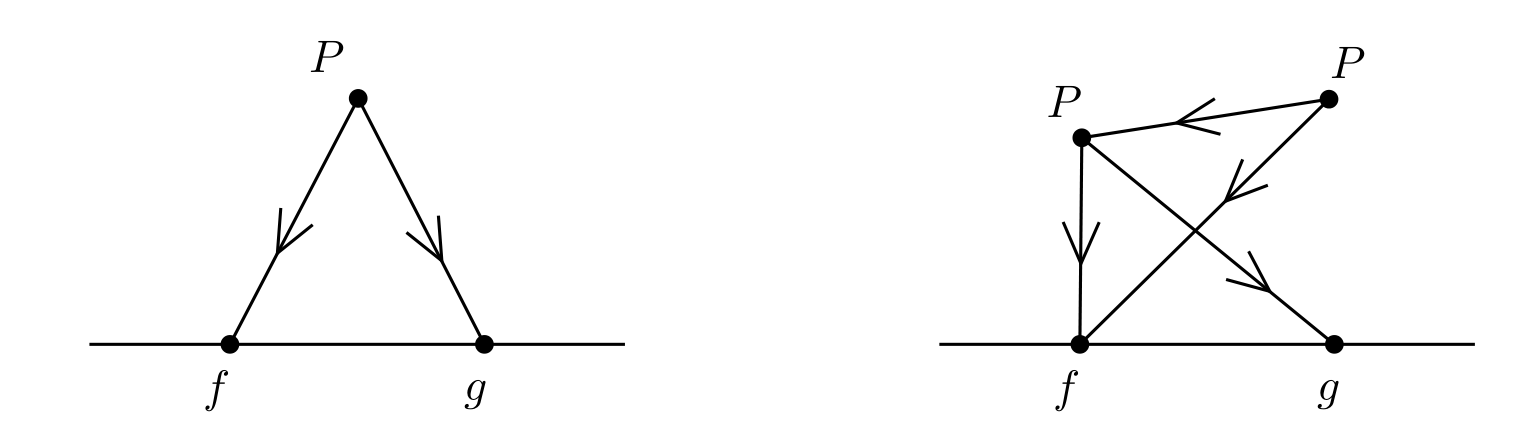
\includegraphics[width=0.68\textwidth]{figures/fig_p320_a.png}
\end{center}
% [图：原书 p.320，图内文字照原样保留]

从每个 $\Gamma_r$ 都可以写出一个双微分算子 $C_{\Gamma_r}(f,g)$：对内部的每个顶点，把 $P=\frac12\sum_{i,j}P^{ij}(\mathbf x)\frac{\partial}{\partial x^i}\otimes\frac{\partial}{\partial x^j}$ 分配给该顶点，并把两个导数 $\frac{\partial}{\partial x^i}$ 与 $\frac{\partial}{\partial x^j}$ 分配给它的两条出边。例如，上图中的第一个图给出
\[
\frac12\sum_{i,j}P^{ij}(\mathbf x)\frac{\partial f}{\partial x^i}
\otimes\frac{\partial g}{\partial x^j},
\]
第二个图给出
\[
\frac12\sum_{i,j}P^{ij}\sum_{k,m}\frac12
\Bigl(\frac{\partial}{\partial x^i}P^{km}\Bigr)
\frac{\partial^2f}{\partial x^k\partial x^j}\frac{\partial g}{\partial x^m}.
\]
于是可以构造如下形式的星乘积
\[
\mu_r(f,g)=\sum_{\Gamma_r}\omega_{\Gamma_r}C_{\Gamma_r}(f,g),
\]
其中系数 $\omega_{\Gamma_r}$ 来自上半平面构型空间上适当的费曼图积分。

费曼图积分来自泊松 $\sigma$-模型中的关联函数
\[
S[X,\eta]=\int_H\eta_idx^i+\frac12\int_HP^{ij}(x)\eta_i\wedge\eta_j,
\]
其中 $X=(X^i)$ 是描述从上半平面 $H$ 到 $\R^n$ 的映射的玻色场
\[
X:H\longrightarrow\R^n
\]

% [原文 p.321]
而 $\eta=(\eta_i)$ 是取值在 $H$ 上、作为 $1$-形式的费米场。星乘积 $\ast$ 的结合性由斯托克斯定理的一个变体推出。

Moyal 乘积公式对应图
\begin{center}
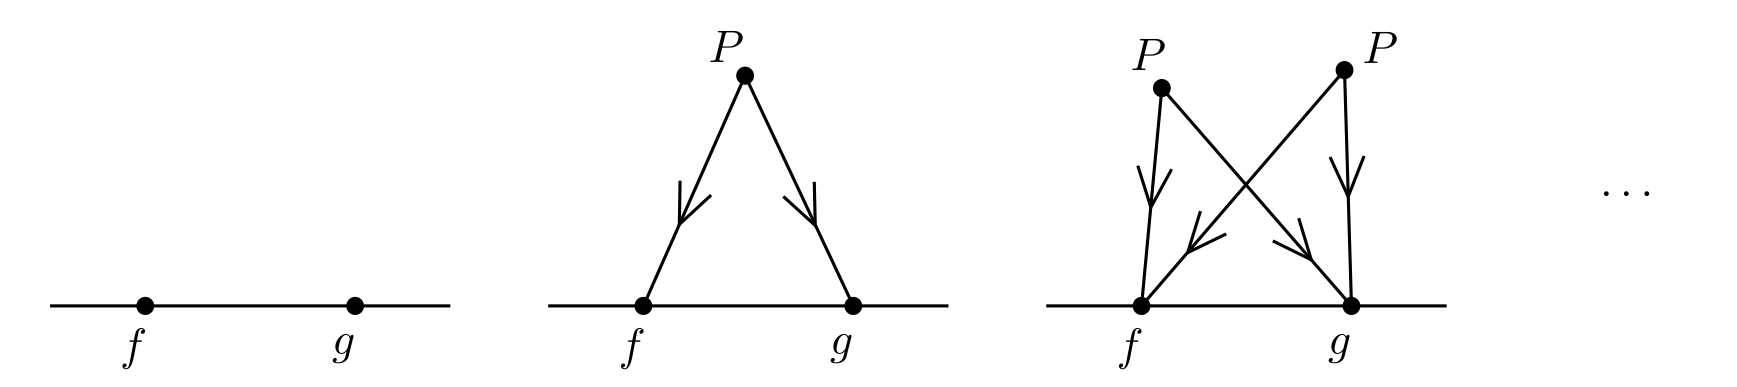
\includegraphics[width=0.75\textwidth]{figures/fig_p321_a.png}
\end{center}
% [图：原书 p.321，图内文字照原样保留]

孔采维奇的公式通过所有可能的、边连接两个内部顶点的图，给出 Moyal 乘积的一个显式修正。
\begin{center}
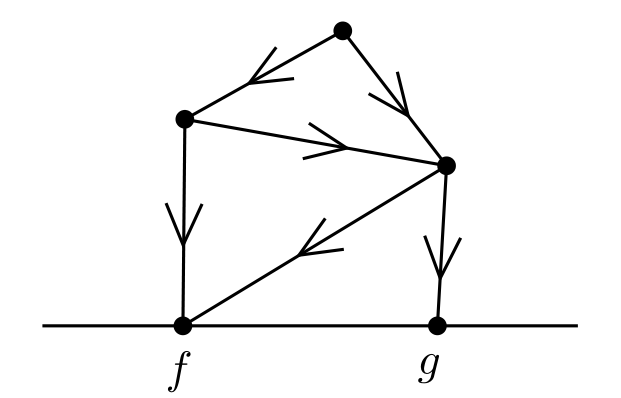
\includegraphics[width=0.42\textwidth]{figures/fig_p321_b.png}
\end{center}
% [图：原书 p.321，图内文字照原样保留]

\takeaway{本节引入泊松流形与泊松上同调，用多向量场和斯豪滕–奈恩黑斯括号刻画泊松结构；随后定义星乘积，并概述孔采维奇用图展开构造形变量子化的基本思路。}

\section{迹映射}

本节中我们考虑辛流形 $(M,\omega)$。设 $(C^\infty(M)[[\lambda]],\star)$ 是形变量子化。若一个 $\lambda$-线性映射
\[
\operatorname{Tr}:C^\infty(M)[[\lambda]]\longrightarrow\R((\lambda))
\]
对任意 $f,g\in C^\infty(M)[[\lambda]]$ 满足
\[
\operatorname{Tr}(f\star g)=\operatorname{Tr}(g\star f),
\qquad\text{或等价地}\qquad
\operatorname{Tr}([f,g]_\star)=0,
\]
则称它为迹映射。由于 $\operatorname{Tr}$ 是 $\lambda$-线性的，只需假设 $f,g\in C^\infty(M)$。

星乘积 $\star$ 描述相空间上量子化算子的代数结构。若存在量子化算子的表示，则相应希尔伯特空间上的迹会湮灭算子交换子。上面定义的迹映射恰好在不指定表示的情况下刻画了这一信息。

事实证明，在辛流形上，形变量子化代数上存在唯一的非平凡迹映射（相差常数倍）。本节我们借助 §2.8.5 中的量子霍赫希尔德–科斯坦特–罗森伯格（HKR）映射以及费多谢夫的阿贝尔联络，给出这个迹映射的显式构造。

% [原文 p.322]
\subsection{微分分次代数}

\paragraph{微分分次代数（DGA）}\par

\begin{definition}{6.4.1}
  微分分次代数（DGA）由分次向量空间
  \[
  A=\bigoplus_{n\in\Z}A^n
  \]
  以及结合乘积 $\cdot$ 与线性映射 $d:A\to A$（微分）组成，满足
  \begin{enumerate}[label=(\arabic*),leftmargin=3.2em,itemsep=1pt]
    \item 乘积 $\cdot$ 保持次数：$A^m\cdot A^n\subseteq A^{m+n}$；
    \item 微分 $d$ 把次数加一：$d:A^n\to A^{n+1}$，且 $d^2=0$；
    \item 分次莱布尼茨律成立：对任意 $a_1,a_2\in A$，
    \[
    d(a_1\cdot a_2)=d(a_1)\cdot a_2+(-1)^{|a_1|}a_1\cdot d(a_2).
    \]
  \end{enumerate}
\end{definition}

这里 $|a|$ 表示 $a$ 的次数，即当 $a\in A^p$ 时 $|a|=p$。

对分次代数 $A$，我们用 $[-,-]$ 表示分次交换子
\[
[a_1,a_2]:=a_1a_2-(-1)^{|a_1||a_2|}a_2a_1.
\]
若对任意 $a_1,a_2\in A$ 都有 $[a_1,a_2]=0$，则称 $A$ 分次交换。

\begin{example}{6.4.2}
  流形 $M$ 上的德拉姆复形 $(\Omega^\bullet(M),d)$ 是 DGA。微分 $d$ 是德拉姆微分。$\Omega^\bullet(M)$ 分次交换。
\end{example}

\begin{example}{6.4.3}
  设 $(V,\omega)$ 是带线性坐标 $\{y^i\}$ 的线性辛空间。令
  \[
  \widehat\Omega(V):=\R[[y^i,dy^i,\lambda]]
  \]
  表示 $V$ 上取值在 $\R[[\lambda]]$ 中的形式微分形式。设 $\hat d$ 表示关于变量 $\{y^i\}$ 的德拉姆微分
  \[
  \hat d=\sum_idy^i\frac{\partial}{\partial y^i}.
  \]
  Moyal 乘积 $\star$ 通过
  \[
  (f_I(y,\lambda)dy^I)\star(g_J(y,\lambda)dy^J)
  :=(f_I(y,\lambda)\star g_J(y,\lambda))dy^I\wedge dy^J
  \]
  延拓为 $\widehat\Omega(V)$ 上的乘积。这里 $I,J$ 是多重组指标。三元组 $(\widehat\Omega(V),\star,\hat d)$ 定义了 DGA，§6.4.3 将用它构造迹映射。
\end{example}

% [原文 p.323]
\paragraph{霍赫希尔德链复形}\par

在 §2.8.5 中，我们讨论了结合代数的霍赫希尔德链复形
\[
\cdots\to C_p(A)\xrightarrow{b}C_{p-1}(A)\xrightarrow{b}\cdots
\xrightarrow{b}C_1(A)\xrightarrow{b}C_0(A).
\]
这自然地推广到微分分次代数。我们遵循 [57]。

设 $(A,d)$ 是 DGA，其中 $d$ 是微分，且
\[
C_p(A)=A^{\otimes p+1}.
\]
霍赫希尔德微分 $b$ 修改为带分次符号的形式
\begin{align*}
&b(a_0\otimes a_1\otimes\cdots\otimes a_p)\\
&\quad:=\sum_{k=0}^{p-1}(-1)^{1+\sum_{i=0}^{k}(|a_i|+1)}
a_0\otimes\cdots\otimes a_ka_{k+1}\otimes\cdots\otimes a_p\\
&\qquad+(-1)^{|a_p|+(|a_p|+1)\sum_{i=0}^{p-1}(|a_i|+1)}
a_pa_0\otimes a_1\otimes\cdots\otimes a_{p-1}.
\end{align*}
微分 $d$ 诱导霍赫希尔德链上的微分（仍记作 $d$）
\[
d(a_0\otimes a_1\otimes\cdots\otimes a_p)
:=\sum_{k=0}^{p}(-1)^{\sum_{i=0}^{k-1}(|a_i|+1)}
a_0\otimes\cdots\otimes da_k\otimes\cdots\otimes a_p.
\]
直接验证可得
\[
b^2=d^2=0,\qquad bd+db=0.
\]

链复形 $C_\bullet(A)$ 是双分次的。一个分次 $p$ 是霍赫希尔德次数 $C_p(A)$。另一个内部分次 $q$ 来自 $A$ 的分次张量：
\[
C_p(A)_q=\bigoplus_{j_0+\cdots+j_p=q}
A^{j_0}\otimes A^{j_1}\otimes\cdots\otimes A^{j_p}.
\]
我们有
\begin{align*}
b&:C_p(A)_q\longrightarrow C_{p-1}(A)_q,\\
d&:C_p(A)_q\longrightarrow C_p(A)_{q+1}.
\end{align*}
DGA $(A,d)$ 的霍赫希尔德链复形成为双复形 $C_\bullet(A)$ 以 $d+b$ 为微分的总复形。

下面引入霍赫希尔德链上的几个运算，它们将会有用。

\begin{definition}{6.4.4}
  给定 $a\in A$，定义
  \[
  \operatorname{ad}_a:A\longrightarrow A,
  \qquad
  \operatorname{ad}_a(u):=[a,u]=au-(-1)^{|a||u|}ua,
  \]
  并把 $\operatorname{ad}_a$ 延拓到霍赫希尔德链
  \[
  \operatorname{ad}_a:C_\bullet(A)\longrightarrow C_\bullet(A),
  \]
  即
  \[
  \operatorname{ad}_a(a_0\otimes a_1\otimes\cdots\otimes a_p)
  =\sum_{k=0}^{p}(-1)^{|a|\sum_{i=0}^{k-1}(|a_i|+1)}
  a_0\otimes\cdots\otimes\operatorname{ad}_aa_k\otimes\cdots\otimes a_p.
  \]
\end{definition}

% [原文 p.324]
例如，有
\[
\operatorname{ad}_a(a_0\otimes a_1)
=[a,a_0]\otimes a_1+(-1)^{|a|(|a_0|+1)}a_0\otimes[a,a_1].
\]

\begin{definition}{6.4.5}
  给定 $a\in A$，定义
  \[
  \Lambda_a:C_\bullet(A)\longrightarrow C_\bullet(A)
  \]
  如下：
  \[
  \Lambda_a(a_0\otimes a_1\otimes\cdots\otimes a_p)
  =\sum_{k=0}^{p}(-1)^{|a|+(|a|+1)\sum_{i=0}^{k}(|a_i|+1)}
  a_0\otimes\cdots\otimes a_k\otimes a\otimes a_{k+1}\otimes\cdots\otimes a_p.
  \]
\end{definition}

例如，有
\[
\Lambda_a(a_0\otimes a_1)
=(-1)^{|a|+(|a|+1)(|a_0|+1)}a_0\otimes a\otimes a_1
+(-1)^{|a|+(|a|+1)(|a_0|+|a_1|+2)}a_0\otimes a_1\otimes a.
\]

\begin{proposition}{6.4.6}
  以下关系成立：
  \begin{align*}
  \operatorname{ad}_{[a,\bar a]}
  &=\operatorname{ad}_a\operatorname{ad}_{\bar a}
  -(-1)^{|a||\bar a|}\operatorname{ad}_{\bar a}\operatorname{ad}_a,\\
  \Lambda_a\Lambda_{\bar a}
  &=(-1)^{(|a|+1)(|\bar a|+1)}\Lambda_{\bar a}\Lambda_a,\\
  \operatorname{ad}_a
  &=b\Lambda_a-(-1)^{|a|+1}\Lambda_ab,\\
  \Lambda_{\operatorname{ad}_a\bar a}
  &=(-1)^{|a|}\bigl(\operatorname{ad}_a\Lambda_{\bar a}
  -(-1)^{|a|(|\bar a|+1)}\Lambda_{\bar a}\operatorname{ad}_a\bigr),\\
  \operatorname{ad}_{da}
  &=d\operatorname{ad}_a-(-1)^{|a|}\operatorname{ad}_ad,\\
  \Lambda_{da}
  &=-\bigl(d\Lambda_a-(-1)^{|a|+1}\Lambda_ad\bigr).
  \end{align*}
\end{proposition}

\begin{proof}
  直接计算。
\end{proof}

\paragraph{扭转构造}\par

设 $a\in A^1$ 是次数 $1$ 的元素。考虑用 $a$ 扭转微分 $d$：
\[
d_a:=d+\operatorname{ad}_a.
\]
这样的 $d_a$ 也满足莱布尼茨律
\[
d_a(a_1\cdot a_2)=(d_aa_1)\cdot a_2+(-1)^{|a_1|}a_1\cdot d_a(a_2).
\]
由命题 6.4.6，有
\[
d_a^2=\operatorname{ad}_{da+\frac12[a,a]}.
\]

\begin{definition}{6.4.7}
  $(A,d)$ 的毛雷尔–嘉当元素是满足
  \[
  da+\frac12[a,a]=0
  \]
  的次数 $1$ 元素 $a\in A^1$。
\end{definition}

这也称为毛雷尔–嘉当方程。由于 $|a|=1$，这与
\[
da+a^2=0
\]
相同。

% [原文 p.325]
于是，若 $a$ 是毛雷尔–嘉当元素，则 $(A,d_a)$ 定义了新的 DGA，称为 $(A,d)$ 经 $a$ 的扭转。扭转后 DGA 的霍赫希尔德链复形与未扭转者的关系由下述命题给出。

\begin{proposition}{6.4.8}
  对任意次数 $1$ 元素 $a\in A^1$，有
  \[
  \ee^{-\Lambda_a}(d+b)\ee^{\Lambda_a}
  =d+b+\operatorname{ad}_a-\Lambda_{da+a^2}.
  \]
  特别地，若 $a$ 是毛雷尔–嘉当元素，则算子 $\ee^{\Lambda_a}$ 在下述意义下把扭转后 $(A,d_a)$ 的霍赫希尔德链复形与未扭转的 $(A,d)$ 缠结起来：
  \[
  (d+b)\ee^{\Lambda_a}=\ee^{\Lambda_a}(d+\operatorname{ad}_a+b).
  \]
\end{proposition}

\begin{proof}
由命题 6.4.6，
\begin{align*}
[d,\Lambda_a]&=-\Lambda_{da},\\
[b,\Lambda_a]&=\operatorname{ad}_a,\\
[\operatorname{ad}_a,\Lambda_a]
&=-\Lambda_{\operatorname{ad}_a(a)}=-2\Lambda_{a^2}.
\end{align*}
由此可知
\begin{align*}
\ee^{-\Lambda_a}(d+b)\ee^{\Lambda_a}
&=(d+b)+[d+b,\Lambda_a]+\frac12\bigl[[d+b,\Lambda_a],\Lambda_a\bigr]\\
&=d+b+\operatorname{ad}_a-\Lambda_{da}-\Lambda_{a^2}.
\end{align*}
\end{proof}

\subsection{量子 HKR 映射}

在 §2.8.5 中，我们说明了相空间 $\R^{2n}$ 上的 $S^1$-关联如何导出量子 HKR 映射。我们在形式外尔代数上重新表述这一构造，并说明如何把它粘合到辛流形上的外尔丛。

\paragraph{局部情形}\par

回忆 §2.8.4 中的 $S^1$-传播子
\[
G(\theta_1,\theta_2)=g(\theta_2-\theta_1)
=\sum_{n\in\Z\setminus\{0\}}\frac{i}{2\pi n}
\ee^{2\pi in(\theta_2-\theta_1)}.
\]
周期函数 $g(\theta)$ 显式为
\[
g(\theta)=
\begin{cases}
0, & \theta=0,\\[2pt]
\theta-\dfrac12, & 0<\theta<1.
\end{cases}
\]
设 $(V,\omega)$ 是线性辛空间，
\[
\omega=\frac12\sum_{i,j}\omega_{ij}dy^i\wedge dy^j.
\]
相应的形式外尔代数是
\[
\widehat{\mathcal W}(V)
=(\mathcal O(V)[[\lambda]],\ast)
=(\R[[y^i,\lambda]],\ast).
\]
下面的定义把定义 2.8.12 改写成当前的框架。

% [原文 p.326]
\begin{definition}{6.4.9}
  定义 $S^1$-关联映射
  \[
  \langle-\rangle_{S^1}:
  \widehat{\mathcal W}(V)\otimes\cdots\otimes\widehat{\mathcal W}(V)
  \longrightarrow\widehat{\mathcal W}(V)
  \]
  如下：
  \begin{align*}
  &\langle f_0\otimes f_1\otimes\cdots\otimes f_m\rangle_{S^1}\\
  &\quad:=m!\int_{\operatorname{Cyc}_{m+1}(S^1)}
  d\theta_0d\theta_1\cdots d\theta_m\\
  &\qquad\times\exp\Bigl(\frac{\lambda}{2}
  \sum_{i,j,\alpha,\beta}\omega^{ij}G(\theta_\alpha,\theta_\beta)
  \frac{\partial}{\partial y_i^{(\alpha)}}
  \frac{\partial}{\partial y_j^{(\beta)}}\Bigr)\\
  &\qquad\times
  f_0(\mathbf y^{(0)},\lambda)\cdots f_m(\mathbf y^{(m)},\lambda)
  \Big|_{y_i^{(\alpha)}=y^i}.
  \end{align*}
  这里
  \[
  \operatorname{Cyc}_{m+1}(S^1)
  =\bigl\{(\theta_0,\theta_1,\cdots,\theta_m)\in(S^1)^{m+1}
  \mid \theta_0,\theta_1,\cdots,\theta_m
  \text{ 按时针循环次序互异}\bigr\}.
  \]
\end{definition}

\begin{center}
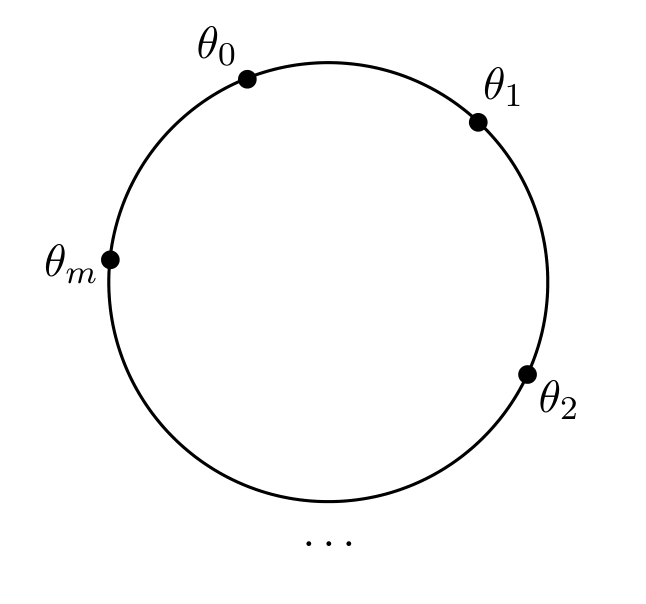
\includegraphics[width=0.30\textwidth]{figures/fig_p326_a.png}
\end{center}
% [图：原书 p.326，图内文字照原样保留]

下面的引理在我们讨论一般辛流形上 $S^1$-关联映射的粘合时会用到。

\begin{lemma}{6.4.10}
  设 $\mathfrak h(\mathbf y)$ 是常数或关于 $\mathbf y$ 线性的。则对任意 $f_i\in\widehat{\mathcal W}(V)$，
  \[
  \sum_{i=0}^{m-1}\langle f_0\otimes\cdots\otimes f_i
  \otimes\mathfrak h\otimes f_{i+1}\otimes\cdots\otimes f_m\rangle_{S^1}
  +\langle f_0\otimes\cdots\otimes f_m\otimes\mathfrak h\rangle_{S^1}
  =\mathfrak h\langle f_0\otimes\cdots\otimes f_m\rangle_{S^1}.
  \]
\end{lemma}

\begin{proof}
当 $\mathfrak h$ 为常数时，这显然成立。设 $\mathfrak h$ 关于 $\mathbf y$ 线性。利用定义 6.4.9 中的显式公式，
\begin{align*}
&\sum_{i=0}^{m-1}\langle f_0\otimes\cdots\otimes f_i
\otimes\mathfrak h\otimes f_{i+1}\otimes\cdots\otimes f_m\rangle_{S^1}
+\langle f_0\otimes\cdots\otimes f_m\otimes\mathfrak h\rangle_{S^1}\\
&\quad=\mathfrak h\langle f_0\otimes\cdots\otimes f_m\rangle_{S^1}
+\text{含 }\int_0^1d\theta_iG(\theta_i,\theta_j)\text{ 的项}.
\end{align*}
命题由下述观察得到：
\[
\int_0^1d\theta_iG(\theta_i,\theta_j)
=\int_0^1d\theta\Bigl(\theta-\frac12\Bigr)=0.
\]
\end{proof}

记
\[
\widetilde\Omega(V):=\R[[y^i,dy^i,\lambda]].
\]
它表示 $V$ 上取值于 $\R[[\lambda]]$ 的形式微分形式。

% [原文 p.327]
令
\[
\widehat d=\sum_i dy^i\frac{\partial}{\partial y^i}
\]
表示 $\{y^i\}$ 中的德拉姆微分。

\begin{definition}{6.4.11}
  我们定义量子 HKR 映射
  \[
  \rho^\lambda:\widehat{\mathcal W}(V)\otimes\cdots\otimes\widehat{\mathcal W}(V)
  \longrightarrow\widehat\Omega(V)
  \]
  为
  \[
  \rho^\lambda(f_0\otimes f_1\otimes\cdots\otimes f_m)
  =\frac{1}{m!}
  \bigl\langle f_0\otimes\widehat df_1\otimes\cdots\otimes\widehat df_m
  \bigr\rangle_{S^1}.
  \]
  这里 $\widehat df=\sum_i\partial_{y^i}f\,dy^i$，并且
  \begin{align*}
  &\bigl\langle f_0\otimes\widehat df_1\otimes\cdots\otimes\widehat df_m
  \bigr\rangle_{S^1}\\
  &\quad:=\sum_{i_1,\cdots,i_m}
  \bigl\langle f_0\otimes\partial_{y^{i_1}}f_1\otimes\cdots
  \otimes\partial_{y^{i_m}}f_m\bigr\rangle_{S^1}
  dy^{i_1}\wedge\cdots\wedge dy^{i_m}.
  \end{align*}
\end{definition}

\begin{proposition}{6.4.12}
  量子 HKR 映射是链映射
  \[
  \rho^\lambda:(C_\bullet(\widehat{\mathcal W}(V)),b)
  \longrightarrow(\widehat\Omega^\bullet(V),\lambda\Delta).
  \]
  这里
  \[
  \Delta=\sum_{i,j}\omega^{ij}\frac{\partial}{\partial y^i}
  \iota_{\partial y^j}
  \]
  是关于泊松双向量 $\omega^{-1}$ 的李导数。
\end{proposition}

\begin{proof}
  证明与 §2.8.5 相同。
\end{proof}

\paragraph{整体情形}\par

设 $(M,\omega)$ 是辛流形，$\nabla$ 是辛联络。设 $\mathcal W=\mathcal W(M)$ 是外尔丛，类似地定义 $TM$ 上形式微分形式的丛
\[
\widehat\Omega=\widehat\Omega(TM)
:=\prod_{k=0}^{\infty}\operatorname{Sym}^k(T^*M)
\otimes\wedge^\bullet T^*M[[\lambda]].
\]
我们还定义 $\mathcal W$ 的霍赫希尔德链丛 $C_\bullet(\mathcal W)$，它在 $p\in M$ 处的纤维是 $\widehat{\mathcal W}(T_pM)$ 的霍赫希尔德链，即
\[
C_p(\mathcal W):=
\Bigl(\prod_{k=0}^{\infty}\operatorname{Sym}^k(T^*M)[[\lambda]]\Bigr)^{\otimes p+1}.
\]
霍赫希尔德微分 $b$ 给出丛映射
\[
b:C_p(\mathcal W)\longrightarrow C_{p-1}(\mathcal W),
\]
而 $(C_\bullet(\mathcal W),b)$ 构成丛的链复形。

纤维式的量子 HKR 映射给出丛的复形的链映射
\[
\rho^\lambda:(C_\bullet(\mathcal W),b)
\longrightarrow(\widehat\Omega^\bullet,\lambda\Delta).
\]

% [原文 p.328]
这里 $\Delta$ 是纤维式的 BV 算子，其局部坐标表示为
\[
\Delta=\sum_{i,j}\omega^{ij}(\mathbf x)
\frac{\partial}{\partial y^i}\iota_{\partial y^j}.
\]
作为丛映射，$b$、$\Delta$ 与 $\rho^\lambda$ 都是 $C^\infty(M)$-线性的。

辛联络 $\nabla$ 还通过张量构造在 $\widehat\Omega$ 上诱导一个联络（仍记为 $\nabla$）。由于 $\omega$ 关于 $\nabla$ 平行，$b$ 与 $\Delta$ 都关于 $\nabla$ 平行：
\[
\nabla(b)=\nabla(\Delta)=0.
\]
由于 $\rho^\lambda$ 由 $\omega$ 与 $S^1$-传播子 $G(\theta_1,\theta_2)$ 构造，我们知道 $\rho^\lambda$ 也关于 $\nabla$ 平行。于是有交换图
\[
\begin{array}{ccc}
C_p(\mathcal W) & \xrightarrow{\ \rho^\lambda\ } & \widehat\Omega^p\\[14pt]
\underset{b}{\Big\downarrow} & & \underset{\lambda\Delta}{\Big\downarrow}\\[14pt]
C_{p-1}(\mathcal W) & \xrightarrow{\ \rho^\lambda\ } & \widehat\Omega^{p-1}
\end{array}
\]
图中所有映射都是关于 $\nabla$ 平行的丛映射。

\subsection{费多谢夫阿贝尔联络的扭转}

设 $D=\nabla+\frac1\lambda[\gamma,-]_\ast$ 是定理 6.2.7 中的费多谢夫阿贝尔联络。它在 $\mathcal W$ 上给出平坦联络，并延拓为
\[
D:\Omega^\bullet(M,\mathcal W)\longrightarrow\Omega^{\bullet+1}(M,\mathcal W),
\]
延拓由下述莱布尼茨律决定：
\[
D(\alpha\otimes s)=d\alpha\otimes s+(-1)^{|p|}\alpha\wedge\nabla s,
\qquad \alpha\in\Omega^p(M),\ s\in\mathcal W.
\]
$D$ 的平坦性推出 $D^2=0$ 在 $\Omega^\bullet(M,\mathcal W)$ 上成立。于是得到复形
\[
(\Omega^\bullet(M,\mathcal W),D),
\]
称为取值于 $\mathcal W$ 的德拉姆复形。

由于 $D$ 与纤维式的 Moyal 乘积相容，$(\Omega^\bullet(M,\mathcal W),D)$ 成为 DGA，其中 $\Omega^p(M,\mathcal W)$ 是次数 $p$ 的部分。把这个 DGA 记为
\[
\Omega(M,\mathcal W):=(\Omega^\bullet(M,\mathcal W),D).
\]
于是按 §6.4.1 得到霍赫希尔德链复形
\[
C_\bullet(\Omega(M,\mathcal W),D+b).
\]
令
\[
\widehat d:\widehat\Omega^\bullet\longrightarrow\widehat\Omega^{\bullet+1}
\]
表示纤维式的德拉姆微分。

% [原文 p.329]
局部坐标为
\[
\widehat d=\sum_i dy^i\frac{\partial}{\partial y^i}.
\]
这个 $\widehat d$ 是丛映射，并且与纤维式的 Moyal 乘积相容：
\[
\widehat d(s_1\ast s_2)=\widehat d(s_1)\ast s_2+s_1\ast\widehat d(s_2),
\qquad \forall\, s_1,s_2\in\mathcal W.
\]
我们把 $\widehat d$ 延拓为 $C^\infty(M)$-线性映射
\[
\widehat d:\Omega^\bullet(M,\widehat\Omega^\bullet)
\longrightarrow\Omega^\bullet(M,\widehat\Omega^{\bullet+1}),
\]
延拓由
\[
\widehat d(\alpha\otimes u)=(-1)^p\alpha\otimes\widehat du,
\qquad \alpha\in\Omega^p(M),\ u\in\widehat\Omega^\bullet
\]
给出。

令
\[
\nabla:\Omega^\bullet(M,\widehat\Omega^\bullet)
\longrightarrow\Omega^{\bullet+1}(M,\widehat\Omega^\bullet)
\]
是辛联络 $\nabla$ 在张量上诱导的映射。设 $\{x^i\}$ 是 $M$ 上的局部坐标，$\{y^j\}$ 是 $TM$ 上诱导的纤维坐标。设联络 $\nabla$ 的作用为
\[
\nabla y^i=\sum_j\alpha^i_j(\mathbf x)y^j,
\]
则
\[
\nabla dy^i=\sum_j\alpha^i_j(\mathbf x)dy^j
=-\widehat d\Bigl(\sum_j\alpha^i_j(\mathbf x)y^j\Bigr)
=-\widehat d\nabla y^i.
\]
把这一计算稍加推广即得
\[
\nabla\widehat d+\widehat d\nabla=0
\qquad\text{在 }\Omega^\bullet(M,\widehat\Omega^\bullet)\text{ 上},
\]
这不过说明 $\widehat d$ 关于 $\nabla$ 平行。

类似地，我们把 BV 算子 $\Delta$ 延拓为
\[
\Delta:\Omega^\bullet(M,\widehat\Omega^\bullet)
\longrightarrow\Omega^\bullet(M,\widehat\Omega^{\bullet-1}),
\]
延拓由
\[
\Delta(\alpha\otimes u)=(-1)^{|p|}\alpha\otimes\Delta u,
\qquad \alpha\in\Omega^p(M),\ u\in\widehat\Omega^\bullet
\]
给出。于是 $\Delta$ 与辛联络 $\nabla$ 相容，即
\[
\nabla\Delta+\Delta\nabla=0
\qquad\text{在 }\Omega^\bullet(M,\widehat\Omega^\bullet)\text{ 上}.
\]
我们再把量子 HKR 映射 $\rho^\lambda:C_\bullet(\mathcal W)\to\widehat\Omega^\bullet$ 延拓为取值于 $\Omega^\bullet(M)$ 的映射
\[
\rho^\lambda:C_\bullet(\Omega(M,\mathcal W))
\longrightarrow\Omega(M,\widehat\Omega^\bullet),
\]
延拓由
\[
\rho^\lambda(\alpha_0u_0\otimes\alpha_1u_1\otimes\cdots\otimes\alpha_mu_m)
:=(-1)^{\sum_{k=1}^{m-1}k|\alpha_k|}
(\alpha_0\wedge\cdots\wedge\alpha_m)\rho^\lambda(u_0\otimes\cdots\otimes u_m)
\]
给出。

% [原文 p.330]
这里 $\alpha_i\in\Omega^{|\alpha_i|}(M)$，$u_i\in\mathcal W$。下述图表交换：
% [图：原书 p.330，交换图按原文重绘，图内仅有数学标注；原图无题注]
\begin{center}
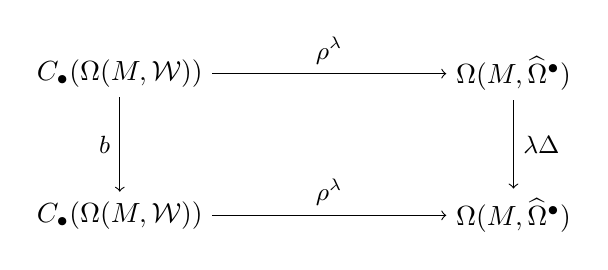
\begin{tikzpicture}
\node (A) at (0,0) {$C_\bullet(\Omega(M,\mathcal W))$};
\node (B) at (5.0,0) {$\Omega(M,\widehat\Omega^\bullet)$};
\node (C) at (0,-1.8) {$C_\bullet(\Omega(M,\mathcal W))$};
\node (D) at (5.0,-1.8) {$\Omega(M,\widehat\Omega^\bullet)$};
\draw[->] (A) -- node[above,font=\small] {$\rho^\lambda$} (B);
\draw[->] (C) -- node[above,font=\small] {$\rho^\lambda$} (D);
\draw[->] (A) -- node[left,font=\small] {$b$} (C);
\draw[->] (B) -- node[right,font=\small] {$\lambda\Delta$} (D);
\end{tikzpicture}
\end{center}

现在可以并入费多谢夫的阿贝尔联络 $D=\nabla+\frac1\lambda[\gamma,-]_\ast$。考虑用 $\gamma\in\Omega^1(M,\mathcal W)$ 扭转霍赫希尔德链：
\[
e^{\Lambda_{\gamma/\lambda}}:C_\bullet(\Omega(M,\mathcal W))
\longrightarrow C_\bullet(\Omega(M,\mathcal W))[\lambda^{-1}].
\]
这里 $[\lambda^{-1}]$ 表示把 $\lambda$ 局部化：
\[
(-)[\lambda^{-1}]:=(-)\otimes_{\R[[\lambda]]}\R((\lambda)).
\]
由与命题 6.4.8 相同的计算，
\begin{align*}
e^{-\Lambda_{\gamma/\lambda}}(\nabla+b)e^{\Lambda_{\gamma/\lambda}}
&=\nabla+b+\operatorname{ad}_{\gamma/\lambda}
-\Lambda_{\nabla(\gamma/\lambda)+\gamma/\lambda\ast\gamma/\lambda}\\
&=D+b-\frac1\lambda\Lambda_{R_\omega^\nabla+\omega_\lambda}.
\end{align*}
这里用到了定理 6.2.7 中的
\[
\nabla\gamma+\frac{1}{2\lambda}[\gamma,\gamma]_\ast
=R_\omega^\nabla+\omega_\lambda.
\]
因此
\[
e^{\Lambda_{\gamma/\lambda}}(D+b)
=\Bigl(\nabla+b+\frac1\lambda\Lambda_{R_\omega^\nabla+\omega_\lambda}\Bigr)
e^{\Lambda_{\gamma/\lambda}}.
\]

\begin{definition}{6.4.13}
  我们定义费多谢夫扭转的量子 HKR 映射为
  \[
  \rho_D^\lambda:=\rho^\lambda\circ e^{\Lambda_{\gamma/\lambda}}:
  C_\bullet(\Omega(M,\mathcal W))
  \longrightarrow\Omega(M,\widehat\Omega^\bullet)[\lambda^{-1}].
  \]
\end{definition}

下述命题是 [25] [30] 中 BV 量子化结果的重述。

\begin{proposition}{6.4.14}
  下述图表交换：
  % [图：原书 p.330，交换图按原文重绘，图内仅有数学标注；原图无题注]
  \begin{center}
  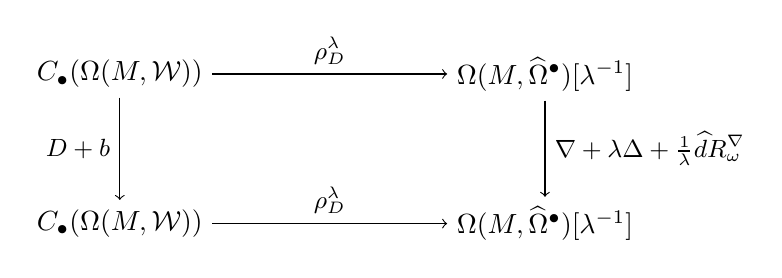
\begin{tikzpicture}
  \node (A) at (0,0) {$C_\bullet(\Omega(M,\mathcal W))$};
  \node (B) at (5.4,0) {$\Omega(M,\widehat\Omega^\bullet)[\lambda^{-1}]$};
  \node (C) at (0,-1.9) {$C_\bullet(\Omega(M,\mathcal W))$};
  \node (D) at (5.4,-1.9) {$\Omega(M,\widehat\Omega^\bullet)[\lambda^{-1}]$};
  \draw[->] (A) -- node[above,font=\small] {$\rho_D^\lambda$} (B);
  \draw[->] (C) -- node[above,font=\small] {$\rho_D^\lambda$} (D);
  \draw[->] (A) -- node[left,font=\small] {$D+b$} (C);
  \draw[->] (B) -- node[right,font=\small]
    {$\nabla+\lambda\Delta+\frac{1}{\lambda}\widehat dR_\omega^\nabla$} (D);
  \end{tikzpicture}
  \end{center}
  等价地，$\rho_D^\lambda$ 给出复形的链映射
  \[
  \rho_D^\lambda:(C_\bullet(\Omega(M,\mathcal W)),D+b)
  \longrightarrow\Bigl(\Omega(M,\widehat\Omega^\bullet)[\lambda^{-1}],
  \nabla+\lambda\Delta+\frac1\lambda\widehat dR_\omega^\nabla\Bigr).
  \]
\end{proposition}

\begin{proof}
  观察到
  \[
  \widehat d(R_\omega^\nabla+\omega_\lambda)=\widehat dR_\omega^\nabla,
  \]
  它关于 $y$ 是线性的。由 $\rho^\lambda$ 的定义与引理 6.4.10 可知
  \[
  \rho^\lambda\circ\Lambda_{R_\omega^\nabla+\omega_\lambda}(-)
  =\widehat dR_\omega^\nabla\cdot\rho^\lambda(-).
  \]

% [原文 p.331]
于是
\begin{align*}
\rho_D^\lambda\circ(D+b)
&=\rho^\lambda\circ e^{\Lambda_{\gamma/\lambda}}\circ(D+b)\\
&=\rho^\lambda\circ\Bigl(\nabla+b+\frac1\lambda
\Lambda_{R_\omega^\nabla+\omega_\lambda}\Bigr)
\circ e^{\Lambda_{\gamma/\lambda}}\\
&=\Bigl(\nabla+\lambda\Delta+\frac1\lambda\widehat dR_\omega^\nabla\Bigr)
\circ\rho^\lambda\circ e^{\Lambda_{\gamma/\lambda}}\\
&=\Bigl(\nabla+\lambda\Delta+\frac1\lambda\widehat dR_\omega^\nabla\Bigr)
\circ\rho_D^\lambda.
\end{align*}
\end{proof}

\subsection{迹映射与指标}

\begin{definition}{6.4.15}
  我们定义丛映射（这里 $\dim M=2n$）
  \[
  \int_{\mathrm{Ber}}:\Omega(M,\widehat\Omega^\bullet)[\lambda^{-1}]
  \longrightarrow\Omega(M)((\lambda))
  \]
  为
  \[
  \int_{\mathrm{Ber}}s(\mathbf x,\mathbf y,\lambda)
  :=\frac{1}{n!}
  \Bigl(\frac12\sum_{i,j}\omega^{ij}(\mathbf x)
  \iota_{\partial y^i}\iota_{\partial y^j}\Bigr)^n
  s\Big|_{\substack{y^i=0\\ dy^i=0}}.
  \]
\end{definition}

\begin{remark}{6.4.16}
  映射 $\int_{\mathrm{Ber}}$ 是格拉斯曼变量上别列津积分的一个版本。

  注意，除非 $s\in\Omega(M,\widehat\Omega^{2n})$，否则 $\int_{\mathrm{Ber}}s=0$。记
  \[
  \widehat\omega:=\frac12\sum_{i,j}\omega_{ij}(\mathbf x)dy^i\wedge dy^j.
  \]
  则对任意 $\alpha\in\Omega(M)$，有
  \[
  \int_{\mathrm{Ber}}\alpha\frac{\widehat\omega^n}{n!}=\alpha.
  \]
\end{remark}

\begin{proposition}{6.4.17}
  $\int_{\mathrm{Ber}}$ 是链映射，它把
  \[
  \int_{\mathrm{Ber}}:
  \Bigl(\Omega(M,\widehat\Omega^\bullet)[\lambda^{-1}],
  \nabla+\lambda\Delta+\frac1\lambda\widehat dR_\omega^\nabla\Bigr)
  \longrightarrow\bigl(\Omega(M)((\lambda)),d\bigr)
  \]
  缠结起来。这里 $d$ 是 $M$ 上的德拉姆微分。
\end{proposition}

\begin{proof}
  对任意 $s\in\Omega(M,\widehat\Omega^\bullet)$，有
  \[
  \int_{\mathrm{Ber}}\Delta(s)=0
  \quad\text{与}\quad
  \int_{\mathrm{Ber}}\widehat dR_\omega^\nabla\wedge s=0,
  \]
  因为 $\Delta(s)$ 不可能落在 $\widehat\Omega^{2n}$ 中，而 $\widehat dR_\omega^\nabla$ 含有 $y$，它在 $\int_{\mathrm{Ber}}$ 下化为零。

  设 $s$ 形如 $s=\alpha\frac{\widehat\omega^n}{n!}$，其中 $\alpha\in\Omega(M)$。由于 $\nabla$ 是辛联络，$\nabla\widehat\omega=0$。于是
  \[
  \int_{\mathrm{Ber}}\nabla\Bigl(\alpha\frac{\widehat\omega^n}{n!}\Bigr)
  =\int_{\mathrm{Ber}}d\alpha\frac{\widehat\omega^n}{n!}
  =d\alpha
  =d\int_{\mathrm{Ber}}\alpha\frac{\widehat\omega^n}{n!}.
  \]
  命题得证。
\end{proof}

% [原文 p.332]
\begin{proposition}{6.4.18}
  费多谢夫扭转的量子 HKR 映射与 $\int_{\mathrm{Ber}}$ 的复合给出链映射
  \[
  \int_{\mathrm{Ber}}\circ\rho_D^\lambda:
  (C_\bullet(\Omega^\bullet(M,\mathcal W)),D+b)
  \longrightarrow(\Omega^\bullet(M)((\lambda)),d).
  \]
\end{proposition}

\begin{proof}
  由命题 6.4.14 与命题 6.4.17 即得。
\end{proof}

回忆 $\mathcal W$ 的平坦截面空间 $\Gamma^{\mathrm{flat}}_D(M,\mathcal W)$ 定义了形变量子化。把 $\int_{\mathrm{Ber}}\circ\rho_D^\lambda$ 限制到 $\Gamma^{\mathrm{flat}}_D(M,\mathcal W)$，得到链映射
\[
\int_{\mathrm{Ber}}\circ\rho_D^\lambda:
(C_\bullet(\Gamma^{\mathrm{flat}}_D(M,\mathcal W)),b)
\longrightarrow(\Omega^\bullet(M)((\lambda)),d).
\]

\begin{definition}{6.4.19}
  在形变量子化代数 $\Gamma^{\mathrm{flat}}_D(M,\mathcal W)$ 上定义迹映射
  \[
  \operatorname{Tr}:\Gamma^{\mathrm{flat}}_D(M,\mathcal W)
  \longrightarrow\R((\lambda))
  \]
  为
  \[
  \operatorname{Tr}(s):=\int_M\int_{\mathrm{Ber}}\rho_D^\lambda(s)
  =\int_M\int_{\mathrm{Ber}}\rho^\lambda\bigl(e^{\Lambda_{\gamma/\lambda}}(s)\bigr).
  \]
\end{definition}

\begin{remark}{6.4.20}
  定义 6.4.19 中处理迹的这一方式等价于 [25, Definition 2.41]。
\end{remark}

\begin{theorem}{6.4.21}
  迹映射 $\operatorname{Tr}$ 满足下述性质：

  \begin{enumerate}[label=(\arabic*),leftmargin=3.2em,itemsep=2pt]
  \item 对 $f\in C^\infty(M)$，
  \[
  \operatorname{Tr}\sigma^{-1}(f)
  =\frac{(-1)^n}{n!\lambda^n}
  \Bigl(\int_Mf\frac{\omega^n}{n!}+O(\lambda)\Bigr).
  \]
  \item 对任意紧支于 $M$ 的 $s_1,s_2\in\Gamma^{\mathrm{flat}}_D(M,\mathcal W)$，
  \[
  \operatorname{Tr}(s_1\ast s_2)=\operatorname{Tr}(s_2\ast s_1).
  \]
  \end{enumerate}
\end{theorem}

\begin{proof}
  对 ①，$\operatorname{Tr}\sigma^{-1}(f)$ 的首阶 $\lambda$-贡献来自
  \begin{align*}
  &\int_M\int_{\mathrm{Ber}}
  \rho^\lambda\bigl(f\otimes(\gamma_0/\lambda)^{\otimes 2n}\bigr)\\
  &\quad=\int_M\int_{\mathrm{Ber}}\frac{1}{(2n)!\lambda^{2n}}
  \Bigl\langle f\otimes
  \underbrace{\widehat d\gamma_0\otimes\cdots\otimes\widehat d\gamma_0}_{2n}
  \Bigr\rangle_{S^1}\\
  &\quad=\frac{1}{(2n)!\lambda^{2n}}
  \int_M\int_{\mathrm{Ber}}
  \bigl(f(\widehat d\gamma_0)^{2n}+O(\lambda)\bigr).
  \end{align*}
  这里
  \[
  \gamma_0=\sum_{i,j}\omega_{ij}dx^iy^j\in\Omega^1(M,\mathcal W),
  \qquad
  \widehat d\gamma_0=-\sum_{i,j}\omega_{ij}dx^idy^j.
  \]
  用达布坐标可直接算出
  \[
  \frac{1}{(2n)!}(\widehat d\gamma_0)^{2n}
  =(-1)^n\frac{\omega^n}{n!}\frac{\widehat\omega^n}{n!}.
  \]
  于是 ① 由
  \begin{align*}
  \frac{1}{(2n)!}\int_M\int_{\mathrm{Ber}}f(\widehat d\gamma_0)^{2n}
  &=\int_M\int_{\mathrm{Ber}}(-1)^nf\frac{\omega^n}{n!}
  \frac{\widehat\omega^n}{n!}\\
  &=(-1)^n\int_Mf\frac{\omega^n}{n!}
  \end{align*}
  得到。

% [原文 p.333]
  对 ②，由命题 6.4.18 有
  \begin{align*}
  \operatorname{Tr}(s_1\ast s_2-s_2\ast s_1)
  &=\operatorname{Tr}\bigl(b(s_1\otimes s_2)\bigr)\\
  &=\int_M\int_{\mathrm{Ber}}\rho_D^\lambda\bigl(b(s_1\otimes s_2)\bigr)\\
  &=\int_Md\int_{\mathrm{Ber}}\rho_D^\lambda(s_1\otimes s_2)=0.
  \end{align*}
\end{proof}

迹映射有一个值得注意的性质：
\[
\operatorname{Tr}(1)=\int_Me^{-\omega_\lambda/\lambda}\hat A(M).
\]
这里 $\omega_\lambda$ 出现在定理 6.2.7 中，它给出形变量子化的参数。这个公式称为代数指标定理，由费多谢夫 [24] 与涅斯特–齐甘 [46] 建立，是阿蒂亚–辛格指标定理的代数类比。计算代数指标的一个几何办法，是使用显式的迹映射（定义 6.4.19），把问题化为用费曼图做的精确半经典计算。这在 [25] [30] 中有说明，而 $\hat A(M)$ 作为单圈贡献出现。

\takeaway{本节构造迹映射：从霍赫希尔德链复形与量子 HKR 映射出发，经费多谢夫阿贝尔联络扭转并与别列津积分复合，得到形变量子化代数上的迹泛函，其首阶给出代数指标定理。}

\chapterreview{本章讨论形变量子化。§6.1 从泊松代数的形式形变出发，说明经典极限恰为泊松括号，并区分严格形变量子化。§6.2 在辛流形上给出费多谢夫的几何构造：外尔丛、辛联络、阿贝尔联络、象征映射与全球化，由此得到闭星乘积。§6.3 转向一般泊松流形，用多向量场与斯豪滕–奈恩黑斯括号刻画泊松结构，引入利赫内罗维奇复形与泊松上同调，并陈述孔采维奇的星乘积。§6.4 建立迹映射：霍赫希尔德链复形、量子 HKR 映射、按费多谢夫联络扭转、别列津积分，最终得到迹泛函与代数指标定理。}











